%% ma: L12-B02-0005
%% lop: 12
%% chuong: 1
%% bai: 2
%% dang: 12.2.4
%% loai: TN4
%% muc: TH
%% dap_an: "C"
%% nguon: "(NBV)-ĐỀ SỐ 5-MỖI NGÀY 1 ĐỀ THI 2025.pdf (D05, MỖI NGÀY 1 ĐỀ - Đề số 5), Phần I Câu 8"
%% kien_thuc: "Bài 2 (giá trị lớn nhất, nhỏ nhất của hàm số trên đoạn, đọc từ bảng biến thiên)"
%% trang_thai: cho-duyet
%% ly_do: "Dạng toán mới đề xuất 12.2.4: giá trị lớn nhất, nhỏ nhất trên đoạn đọc từ bảng biến thiên (tính M+m)"
\begin{ex}
Cho hàm số $y=f(x)$ liên tục trên đoạn $[-2;3]$ và có bảng biến thiên như sau:
\begin{center}
\begin{tikzpicture}
  \tkzTabInit[lgt=1.2,espcl=2.6]{$x$/.8,$y'$/.8,$y$/2}{$-2$,$0$,$1$,$3$}
  \tkzTabLine{,+,0,-,0,+,}
  \tkzTabVar{-/$-8$,+/$-3$,-/$-4$,+/$-2$}
\end{tikzpicture}
\end{center}
Gọi $M$ và $m$ lần lượt là giá trị lớn nhất và giá trị nhỏ nhất của hàm số đã cho trên đoạn $[-2;3]$. Giá trị của $M+m$ bằng
\choice{$-7$}{$-11$}{\True $-10$}{$-6$}
\loigiai{Từ bảng biến thiên, các giá trị cần so sánh là $f(-2)=-8$, $f(0)=-3$, $f(1)=-4$, $f(3)=-2$. Suy ra $M=f(3)=-2$ và $m=f(-2)=-8$. Vậy $M+m=-10$.}
\end{ex}
